% !TEX encoding = UTF-8 Unicode
\documentclass[a4paper]{article}
\usepackage{caption}
\usepackage{subcaption}
\usepackage{textcomp}
\usepackage{paralist}
\usepackage{wrapfig}%https://preview.overleaf.com/public/nhgtcfbqhdqd/images/c3261aacf075202acb6214f8591bc9962a3b8c8b.jpeg
\usepackage{url}
\usepackage{mathtools}
\DeclarePairedDelimiter{\abs}{\lvert}{\rvert}

\usepackage{paralist}
\usepackage{amsfonts}
\usepackage[margin=1in]{geometry}
\usepackage{blindtext}
\usepackage{scrextend}
\usepackage{tikz}
\usetikzlibrary{arrows.meta}
\usepackage{dirtree}
\usepackage{courier}
\usepackage[T1]{fontenc}     % För svenska bokstäver
\usepackage[utf8]{inputenc}  % Teckenkodning UTF8
\usepackage[english, swedish]{babel}  % För svensk avstavning och svenskahttps://preview.overleaf.com/public/nhgtcfbqhdqd/images/c3261aacf075202acb6214f8591bc9962a3b8c8b.jpeghttps://preview.overleaf.com/public/nhgtcfbqhdqd/images/c3261aacf075202acb6214f8591bc9962a3b8c8b.jpeg
\usepackage{listings}
\usepackage{color}
\usepackage{minted}
\usepackage{amsthm}
\usepackage[english]{algorithm2e}
\usepackage{tikz}
\usepackage[pdf]{graphviz}



 
\newcommand{\DomRel}[2]{#1\;\underline{\texttt{>>}}\;#2}
\newcommand{\DomRelStrict}[2]{#1\;\texttt{>>}\;#2}
                             % rubriker (t ex "Innehållsförteckning")
\usepackage{fancyvrb}        % För programlistor med tabulatorer
\fvset{tabsize=4}            % Tabulatorpositioner
\fvset{fontsize=\small}      % Lagom storlek för programlistor

\usepackage{framed}

\title{Design of Flow Analysis}
\author{Hampus Balldin, Emil Hammarström
}

\newcommand {\cat }{%
\mathbf%
}
\newcommand {\domain } [ 1 ] {%
\mathrm{dom}(#1)%
}
\newcommand {\codomain } [ 1 ] {%
\mathrm{cod}(#1)%
}
\newcommand {\idarrow} [ 1 ] [ ] {%
\mathbf{1} {#1}%
}
% Paket:
\usepackage{graphicx}         % För att inkludera bilder.

% Kommandon i denna rapport
\newcommand{\code}[1]{\texttt{#1}} % För programkod i text.
% *** Slut på tillägg för denna rapport. ***

\newcommand{\NL}[0]{ \hfill\\\noindent }
\newenvironment{nscenter}
 {\parskip=0pt\par\nopagebreak\centering}
 {\par\noindent\ignorespacesafterend}
 
\begin{document}              % Början på dokumentet
\selectlanguage{english}
\thispagestyle{empty}


\maketitle                    % Skriver ut rubriken som vi
                              % definierade ovan med \title, \author
                              % och eventuellt \date
\pagenumbering{gobble}
\newpage
\tableofcontents
\pagenumbering{arabic}
\newpage
\section{Introduction}
\subsubsection{Assumptions}
We assume the absence of type errors. For example, one may not evaluate $x + 1$ where $x$ is a Bool.\NL\NL
We assume that the variables are renamed and that PHI-functions are inserted to put the CFG on SSA form.

\subsubsection{CFG IR (Task 1)}
Our CFG IR consists of nodes and edges. An edge between two nodes $n_1$, $n_2$ means that the program execution may continue to $n_2$ after $n_1$. A node is one of the following types:

\begin{minted}{haskell}
data Node = DEF Identifier Expr
		  | BRANCH Expr
	      | RETURN Expr
          | EMPTY
\end{minted}
\noindent
The node relation is kept in a separate data structure that can be queried for successors $S\;n = \{ \text{Successor of } n \}$. Every node (apart from the exit node (Exit)) has at least one successor. 

\paragraph{DEF Node}\NL
A <DEF $i$ $e$> node defines a variable $i$ to take the value of expression $e$. 

\paragraph{BRANCH Node}\NL
\textit{A branch node has two successors. One of them is the ``True''-successor.} \NL
In a <BRANCH $e$> node, the flow continues to the ``True''-successor if $e$ evaluates to True (else the flow continues along the other edge).

\paragraph{RETURN Node}\NL
A <RETURN $e$> node acts like a ``goto Exit'' node. Before going to Exit, the expression $e$ is evaluated. The flow gets absorbed at Exit since Exit has no successors.

\paragraph{EMPTY Node}\NL
An <EMPTY> node acts like a ``no-operation''. We keep it for ease of constructing the CFG.

\NL The three important control-flow structures are IF, WHILE, TWICE. 

\paragraph{IF Construct}\NL
The IF construct uses the BRANCH primitive. A value (\textbf{If} $e\;th\;el$) :: If Expr Stmt Stmt gets transformed into the CFG IR by adding a <BRANCH $e$> node and adding the transformation of $th$ and $el$ as successors in the CFG. 
For ease of construction, we add an <EMPTY> node to the successor sets of $th$ and $el$.

\NL The result of transformation of the statement: \textbf{If COND Skip Skip} is shown in figure \ref{ifflow}.
\begin{figure}[ht!]
\centering	
\scalebox{.7}{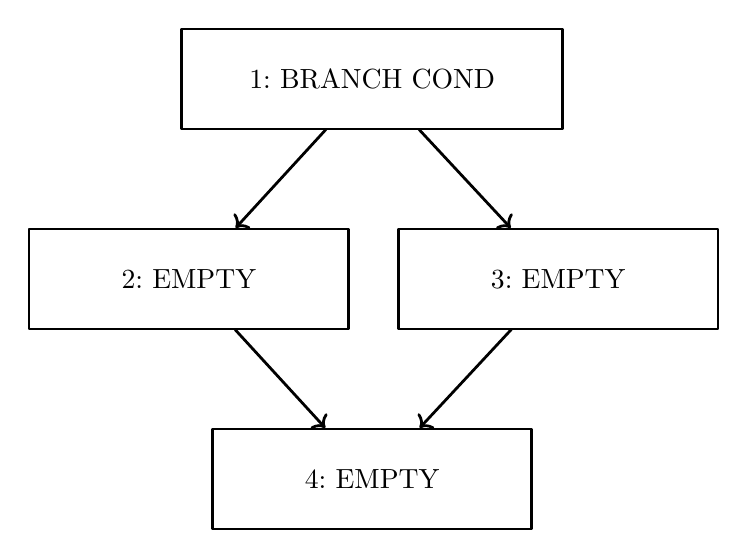
\begin{tikzpicture}[line join=bevel,]
\pgfsetlinewidth{1bp}
%%
\begin{scope}
\pgfsetstrokecolor{black}
\definecolor{strokecol}{rgb}{1.0,1.0,1.0};
\pgfsetstrokecolor{strokecol}
\definecolor{fillcol}{rgb}{1.0,1.0,1.0};
\pgfsetfillcolor{fillcol}
\filldraw (0.0bp,0.0bp) -- (0.0bp,180.0bp) -- (248.0bp,180.0bp) -- (248.0bp,0.0bp) -- cycle;
\end{scope}
\pgfsetcolor{black}
% Edge: 1 -> 2
\draw [->] (106.85bp,143.83bp) .. controls (99.089bp,135.37bp) and (89.72bp,125.15bp)  .. (74.379bp,108.41bp);
% Edge: 3 -> 4
\draw [->] (173.59bp,71.831bp) .. controls (165.72bp,63.369bp) and (156.21bp,53.149bp)  .. (140.63bp,36.413bp);
% Edge: 1 -> 3
\draw [->] (140.41bp,143.83bp) .. controls (148.28bp,135.37bp) and (157.79bp,125.15bp)  .. (173.37bp,108.41bp);
% Edge: 2 -> 4
\draw [->] (74.155bp,71.831bp) .. controls (81.911bp,63.369bp) and (91.28bp,53.149bp)  .. (106.62bp,36.413bp);
% Node: 1
\begin{scope}
\definecolor{strokecol}{rgb}{0.0,0.0,0.0};
\pgfsetstrokecolor{strokecol}
\draw (192.0bp,180.0bp) -- (55.0bp,180.0bp) -- (55.0bp,144.0bp) -- (192.0bp,144.0bp) -- cycle;
\draw (123.5bp,162.0bp) node {1: BRANCH COND};
\end{scope}
% Node: 3
\begin{scope}
\definecolor{strokecol}{rgb}{0.0,0.0,0.0};
\pgfsetstrokecolor{strokecol}
\draw (248.0bp,108.0bp) -- (133.0bp,108.0bp) -- (133.0bp,72.0bp) -- (248.0bp,72.0bp) -- cycle;
\draw (190.5bp,90.0bp) node {3: EMPTY};
\end{scope}
% Node: 2
\begin{scope}
\definecolor{strokecol}{rgb}{0.0,0.0,0.0};
\pgfsetstrokecolor{strokecol}
\draw (115.0bp,108.0bp) -- (0.0bp,108.0bp) -- (0.0bp,72.0bp) -- (115.0bp,72.0bp) -- cycle;
\draw (57.5bp,90.0bp) node {2: EMPTY};
\end{scope}
% Node: 4
\begin{scope}
\definecolor{strokecol}{rgb}{0.0,0.0,0.0};
\pgfsetstrokecolor{strokecol}
\draw (181.0bp,36.0bp) -- (66.0bp,36.0bp) -- (66.0bp,0.0bp) -- (181.0bp,0.0bp) -- cycle;
\draw (123.5bp,18.0bp) node {4: EMPTY};
\end{scope}
%
\end{tikzpicture}
}
\caption{ CFG IR of \textbf{If COND Skip Skip} visualized. }
\label{ifflow}
\end{figure}

\paragraph{WHILE Construct}\NL
The WHILE construct also uses the BRANCH primitive. An empty node is inserted at the false branch to allow nested loops. The last statement in the while body has the <BRANCH e> as its' successor. 

\NL
The branch construct for \textbf{While COND Skip} is shown in figure \ref{whileflow}.

\begin{figure}[ht!]
	\centering	
	\scalebox{.7}{\enlargethispage{100cm}
% Start of code
% \begin{tikzpicture}[anchor=mid,>=latex',line join=bevel,]
\begin{tikzpicture}[line join=bevel,]
  \pgfsetlinewidth{1bp}
%%
\begin{scope}
  \pgfsetstrokecolor{black}
  \definecolor{strokecol}{rgb}{1.0,1.0,1.0};
  \pgfsetstrokecolor{strokecol}
  \definecolor{fillcol}{rgb}{1.0,1.0,1.0};
  \pgfsetfillcolor{fillcol}
  \filldraw (0.0bp,0.0bp) -- (0.0bp,108.0bp) -- (202.0bp,108.0bp) -- (202.0bp,0.0bp) -- cycle;
\end{scope}
  \pgfsetcolor{black}
  % Edge: 2 -> 1
  \draw [->] (74.476bp,36.413bp) .. controls (75.207bp,44.059bp) and (75.42bp,53.108bp)  .. (74.452bp,71.831bp);
  % Edge: 1 -> 2
  \draw [->] (62.548bp,71.831bp) .. controls (61.797bp,64.131bp) and (61.576bp,54.974bp)  .. (62.524bp,36.413bp);
  % Edge: 1 -> 3
  \draw [->] (92.473bp,71.831bp) .. controls (104.29bp,62.878bp) and (118.7bp,51.956bp)  .. (139.54bp,36.163bp);
  % Node: 1
\begin{scope}
  \definecolor{strokecol}{rgb}{0.0,0.0,0.0};
  \pgfsetstrokecolor{strokecol}
  \draw (137.0bp,108.0bp) -- (0.0bp,108.0bp) -- (0.0bp,72.0bp) -- (137.0bp,72.0bp) -- cycle;
  \draw (68.5bp,90.0bp) node {1: BRANCH COND};
\end{scope}
  % Node: 3
\begin{scope}
  \definecolor{strokecol}{rgb}{0.0,0.0,0.0};
  \pgfsetstrokecolor{strokecol}
  \draw (202.0bp,36.0bp) -- (125.0bp,36.0bp) -- (125.0bp,0.0bp) -- (202.0bp,0.0bp) -- cycle;
  \draw (163.5bp,18.0bp) node {3: EMPTY};
\end{scope}
  % Node: 2
\begin{scope}
  \definecolor{strokecol}{rgb}{0.0,0.0,0.0};
  \pgfsetstrokecolor{strokecol}
  \draw (107.0bp,36.0bp) -- (30.0bp,36.0bp) -- (30.0bp,0.0bp) -- (107.0bp,0.0bp) -- cycle;
  \draw (68.5bp,18.0bp) node {2: EMPTY};
\end{scope}
%
\end{tikzpicture}


}
	\caption{ CFG IR of \textbf{If COND Skip Skip} visualized. }
	\label{whileflow}
\end{figure}

\paragraph{TWICE Construct}\NL
The twice construct duplicates a statement in the CFG graph by combining the corresponding transform blocks in sequential order. This has the downside of leading to additional memory usage. On the other hand, the flow analysis is simplified by not introducing additional block types.

\begin{figure}[ht!]
	\centering	
	\scalebox{.6}{\enlargethispage{100cm}
% Start of code
% \begin{tikzpicture}[anchor=mid,>=latex',line join=bevel,]
\begin{tikzpicture}[line join=bevel,]
  \pgfsetlinewidth{1bp}
%%
\begin{scope}
  \pgfsetstrokecolor{black}
  \definecolor{strokecol}{rgb}{1.0,1.0,1.0};
  \pgfsetstrokecolor{strokecol}
  \definecolor{fillcol}{rgb}{1.0,1.0,1.0};
  \pgfsetfillcolor{fillcol}
  \filldraw (0.0bp,0.0bp) -- (0.0bp,252.0bp) -- (293.0bp,252.0bp) -- (293.0bp,0.0bp) -- cycle;
\end{scope}
  \pgfsetcolor{black}
  % Edge: 4 -> 5
  \draw [->] (153.55bp,71.831bp) .. controls (152.8bp,64.131bp) and (152.58bp,54.974bp)  .. (153.52bp,36.413bp);
  % Edge: 2 -> 1
  \draw [->] (70.476bp,180.41bp) .. controls (71.207bp,188.06bp) and (71.42bp,197.11bp)  .. (70.452bp,215.83bp);
  % Edge: 4 -> 6
  \draw [->] (183.47bp,71.831bp) .. controls (195.29bp,62.878bp) and (209.7bp,51.956bp)  .. (230.54bp,36.163bp);
  % Edge: 5 -> 4
  \draw [->] (165.48bp,36.413bp) .. controls (166.21bp,44.059bp) and (166.42bp,53.108bp)  .. (165.45bp,71.831bp);
  % Edge: 3 -> 4
  \draw [->] (159.5bp,143.83bp) .. controls (159.5bp,136.13bp) and (159.5bp,126.97bp)  .. (159.5bp,108.41bp);
  % Edge: 1 -> 2
  \draw [->] (58.548bp,215.83bp) .. controls (57.797bp,208.13bp) and (57.576bp,198.97bp)  .. (58.524bp,180.41bp);
  % Edge: 1 -> 3
  \draw [->] (88.473bp,215.83bp) .. controls (100.29bp,206.88bp) and (114.7bp,195.96bp)  .. (135.54bp,180.16bp);
  % Node: 1
\begin{scope}
  \definecolor{strokecol}{rgb}{0.0,0.0,0.0};
  \pgfsetstrokecolor{strokecol}
  \draw (129.0bp,252.0bp) -- (0.0bp,252.0bp) -- (0.0bp,216.0bp) -- (129.0bp,216.0bp) -- cycle;
  \draw (64.5bp,234.0bp) node {1: BRANCH COND};
\end{scope}
  % Node: 3
\begin{scope}
  \definecolor{strokecol}{rgb}{0.0,0.0,0.0};
  \pgfsetstrokecolor{strokecol}
  \draw (198.0bp,180.0bp) -- (121.0bp,180.0bp) -- (121.0bp,144.0bp) -- (198.0bp,144.0bp) -- cycle;
  \draw (159.5bp,162.0bp) node {3: EMPTY};
\end{scope}
  % Node: 2
\begin{scope}
  \definecolor{strokecol}{rgb}{0.0,0.0,0.0};
  \pgfsetstrokecolor{strokecol}
  \draw (103.0bp,180.0bp) -- (26.0bp,180.0bp) -- (26.0bp,144.0bp) -- (103.0bp,144.0bp) -- cycle;
  \draw (64.5bp,162.0bp) node {2: EMPTY};
\end{scope}
  % Node: 5
\begin{scope}
  \definecolor{strokecol}{rgb}{0.0,0.0,0.0};
  \pgfsetstrokecolor{strokecol}
  \draw (198.0bp,36.0bp) -- (121.0bp,36.0bp) -- (121.0bp,0.0bp) -- (198.0bp,0.0bp) -- cycle;
  \draw (159.5bp,18.0bp) node {5: EMPTY};
\end{scope}
  % Node: 4
\begin{scope}
  \definecolor{strokecol}{rgb}{0.0,0.0,0.0};
  \pgfsetstrokecolor{strokecol}
  \draw (224.0bp,108.0bp) -- (95.0bp,108.0bp) -- (95.0bp,72.0bp) -- (224.0bp,72.0bp) -- cycle;
  \draw (159.5bp,90.0bp) node {4: BRANCH COND};
\end{scope}
  % Node: 6
\begin{scope}
  \definecolor{strokecol}{rgb}{0.0,0.0,0.0};
  \pgfsetstrokecolor{strokecol}
  \draw (293.0bp,36.0bp) -- (216.0bp,36.0bp) -- (216.0bp,0.0bp) -- (293.0bp,0.0bp) -- cycle;
  \draw (254.5bp,18.0bp) node {6: EMPTY};
\end{scope}
%
\end{tikzpicture}


}
	\caption{ CFG IR of \textbf{TWICE (While COND Skip)} visualized. }
	\label{twiceflow}
\end{figure}

%\paragraph{Example Program}\NL
%An example program using the constructs is shown in figure \ref{programexample}. The code used to generate the CFG is included in the appendix.
%
%\begin{figure}[ht!]
%	\centering	
%	\scalebox{.6}{\enlargethispage{100cm}
% Start of code
% \begin{tikzpicture}[anchor=mid,>=latex',line join=bevel,]
\begin{tikzpicture}[line join=bevel,]
  \pgfsetlinewidth{1bp}
%%
\begin{scope}
  \pgfsetstrokecolor{black}
  \definecolor{strokecol}{rgb}{1.0,1.0,1.0};
  \pgfsetstrokecolor{strokecol}
  \definecolor{fillcol}{rgb}{1.0,1.0,1.0};
  \pgfsetfillcolor{fillcol}
\end{scope}
  \pgfsetcolor{black}
  % Edge: 8 -> 9
  \draw [->] (72.519bp,143.83bp) .. controls (73.374bp,136.13bp) and (74.392bp,126.97bp)  .. (76.454bp,108.41bp);
  % Edge: 4 -> 5
  \draw [->] (105.34bp,431.83bp) .. controls (97.349bp,423.37bp) and (87.696bp,413.15bp)  .. (71.89bp,396.41bp);
  % Edge: 3 -> 12
  \draw [->] (239.41bp,503.83bp) .. controls (247.28bp,495.37bp) and (256.79bp,485.15bp)  .. (272.37bp,468.41bp);
  % Edge: 14 -> exit
  \draw [->] (412.85bp,431.83bp) .. controls (417.42bp,423.79bp) and (422.91bp,414.17bp)  .. (433.01bp,396.41bp);
  % Edge: 11 -> 3
  \draw [->] (165.04bp,36.178bp) .. controls (185.66bp,62.23bp) and (219.5bp,112.52bp)  .. (219.5bp,162.0bp) .. controls (219.5bp,378.0bp) and (219.5bp,378.0bp)  .. (219.5bp,378.0bp) .. controls (219.5bp,418.13bp) and (220.68bp,464.54bp)  .. (221.88bp,503.82bp);
  % Edge: start -> 1
  \draw [->] (410.66bp,719.83bp) .. controls (406.3bp,711.79bp) and (401.09bp,702.17bp)  .. (391.47bp,684.41bp);
  % Edge: 4 -> 10
  \draw [->] (125.92bp,431.76bp) .. controls (130.55bp,407.09bp) and (138.84bp,362.86bp)  .. (146.11bp,324.09bp);
  % Edge: 6 -> 7
  \draw [->] (51.509bp,287.83bp) .. controls (51.937bp,280.13bp) and (52.446bp,270.97bp)  .. (53.477bp,252.41bp);
  % Edge: 2 -> 3
  \draw [->] (322.69bp,575.83bp) .. controls (305.23bp,566.45bp) and (283.75bp,554.91bp)  .. (256.3bp,540.16bp);
  % Edge: start -> exit
  \draw [->] (434.7bp,719.6bp) .. controls (453.56bp,693.29bp) and (484.5bp,642.7bp)  .. (484.5bp,594.0bp) .. controls (484.5bp,594.0bp) and (484.5bp,594.0bp)  .. (484.5bp,522.0bp) .. controls (484.5bp,480.15bp) and (468.28bp,433.98bp)  .. (452.2bp,396.17bp);
  % Edge: 7 -> 8
  \draw [->] (58.537bp,215.83bp) .. controls (60.249bp,208.13bp) and (62.283bp,198.97bp)  .. (66.408bp,180.41bp);
  % Edge: 13 -> 14
  \draw [->] (397.27bp,503.83bp) .. controls (398.02bp,496.13bp) and (398.91bp,486.97bp)  .. (400.71bp,468.41bp);
  % Edge: 2 -> 13
  \draw [->] (366.34bp,575.83bp) .. controls (370.7bp,567.79bp) and (375.91bp,558.17bp)  .. (385.53bp,540.41bp);
  % Edge: 12 -> 2
  \draw [->] (297.92bp,468.09bp) .. controls (309.46bp,492.9bp) and (330.3bp,537.68bp)  .. (348.01bp,575.76bp);
  % Edge: 5 -> 6
  \draw [->] (53.491bp,359.83bp) .. controls (53.063bp,352.13bp) and (52.554bp,342.97bp)  .. (51.523bp,324.41bp);
  % Edge: 1 -> 2
  \draw [->] (375.19bp,647.83bp) .. controls (372.49bp,640.05bp) and (369.27bp,630.77bp)  .. (362.89bp,612.41bp);
  % Edge: 9 -> 11
  \draw [->] (96.416bp,71.831bp) .. controls (104.84bp,63.285bp) and (115.04bp,52.944bp)  .. (131.34bp,36.413bp);
  % Edge: 3 -> 4
  \draw [->] (197.27bp,503.83bp) .. controls (184.71bp,494.79bp) and (169.37bp,483.75bp)  .. (147.73bp,468.16bp);
  % Edge: 10 -> 11
  \draw [->] (149.5bp,287.98bp) .. controls (149.5bp,239.29bp) and (149.5bp,104.8bp)  .. (149.5bp,36.009bp);
  % Node: 11
\begin{scope}
  \definecolor{strokecol}{rgb}{0.0,0.0,0.0};
  \pgfsetstrokecolor{strokecol}
  \draw (149.5bp,18.0bp) node {11: EMPTY};
\end{scope}
  % Node: 10
\begin{scope}
  \definecolor{strokecol}{rgb}{0.0,0.0,0.0};
  \pgfsetstrokecolor{strokecol}
  \draw (149.5bp,306.0bp) node {10: EMPTY};
\end{scope}
  % Node: 13
\begin{scope}
  \definecolor{strokecol}{rgb}{0.0,0.0,0.0};
  \pgfsetstrokecolor{strokecol}
  \draw (395.5bp,522.0bp) node {13: EMPTY};
\end{scope}
  % Node: 12
\begin{scope}
  \definecolor{strokecol}{rgb}{0.0,0.0,0.0};
  \pgfsetstrokecolor{strokecol}
  \draw (289.5bp,450.0bp) node {12: EMPTY};
\end{scope}
  % Node: 14
\begin{scope}
  \definecolor{strokecol}{rgb}{0.0,0.0,0.0};
  \pgfsetstrokecolor{strokecol}
  %\draw (456.0bp,468.0bp) -- (349.0bp,468.0bp) -- (349.0bp,432.0bp) -- (456.0bp,432.0bp) -- cycle;
  \draw (402.5bp,450.0bp) node {14: RETURN 0};
\end{scope}
  % Node: 1
\begin{scope}
  \definecolor{strokecol}{rgb}{0.0,0.0,0.0};
  \pgfsetstrokecolor{strokecol}
  \draw (381.5bp,666.0bp) node {1: DEF (x := 0)};
\end{scope}
  % Node: start
\begin{scope}
  \definecolor{strokecol}{rgb}{0.0,0.0,0.0};
  \pgfsetstrokecolor{strokecol}
  \draw (420.5bp,738.0bp) node {Start};
\end{scope}
  % Node: 3
\begin{scope}
  \definecolor{strokecol}{rgb}{0.0,0.0,0.0};
  \pgfsetstrokecolor{strokecol}
  \draw (222.5bp,522.0bp) node {3: BRANCH (x < 20)};
\end{scope}
  % Node: 2
\begin{scope}
  \definecolor{strokecol}{rgb}{0.0,0.0,0.0};
  \pgfsetstrokecolor{strokecol}
  \draw (356.5bp,594.0bp) node {2: BRANCH (x < 10)};
\end{scope}
  % Node: 5
\begin{scope}
  \definecolor{strokecol}{rgb}{0.0,0.0,0.0};
  \pgfsetstrokecolor{strokecol}
  %\draw (109.0bp,396.0bp) -- (0.0bp,396.0bp) -- (0.0bp,360.0bp) -- (109.0bp,360.0bp) -- cycle;
  \draw (54.5bp,378.0bp) node {5: DEF (x := x + 1)};
\end{scope}
  % Node: 4
\begin{scope}
  \definecolor{strokecol}{rgb}{0.0,0.0,0.0};
  \pgfsetstrokecolor{strokecol}
  %\draw (191.0bp,468.0bp) -- (54.0bp,468.0bp) -- (54.0bp,432.0bp) -- (191.0bp,432.0bp) -- cycle;
  \draw (122.5bp,450.0bp) node {4: BRANCH (x == 5)};
\end{scope}
  % Node: 7
\begin{scope}
  \definecolor{strokecol}{rgb}{0.0,0.0,0.0};
  \pgfsetstrokecolor{strokecol}
 % \draw (93.0bp,252.0bp) -- (16.0bp,252.0bp) -- (16.0bp,216.0bp) -- (93.0bp,216.0bp) -- cycle;
  \draw (54.5bp,234.0bp) node {7: EMPTY};
\end{scope}
  % Node: 6
\begin{scope}
  \definecolor{strokecol}{rgb}{0.0,0.0,0.0};
  \pgfsetstrokecolor{strokecol}
 % \draw (89.0bp,324.0bp) -- (12.0bp,324.0bp) -- (12.0bp,288.0bp) -- (89.0bp,288.0bp) -- cycle;
  \draw (50.5bp,306.0bp) node {6: EMPTY};
\end{scope}
  % Node: 9
\begin{scope}
  \definecolor{strokecol}{rgb}{0.0,0.0,0.0};
  \pgfsetstrokecolor{strokecol}
 % \draw (117.0bp,108.0bp) -- (40.0bp,108.0bp) -- (40.0bp,72.0bp) -- (117.0bp,72.0bp) -- cycle;
  \draw (78.5bp,90.0bp) node {9: EMPTY};
\end{scope}
  % Node: 8
\begin{scope}
  \definecolor{strokecol}{rgb}{0.0,0.0,0.0};
  \pgfsetstrokecolor{strokecol}
 % \draw (109.0bp,180.0bp) -- (32.0bp,180.0bp) -- (32.0bp,144.0bp) -- (109.0bp,144.0bp) -- cycle;
  \draw (70.5bp,162.0bp) node {8: EMPTY};
\end{scope}
  % Node: exit
\begin{scope}
  \definecolor{strokecol}{rgb}{0.0,0.0,0.0};
  \pgfsetstrokecolor{strokecol}
  \draw (443.5bp,378.0bp) node {Exit};
\end{scope}
%
\end{tikzpicture}
}
%	\caption{ CFG IR of program example visualized. }
%	\label{programexample}
%\end{figure}

\subsubsection{Skipping WHILE (Task 2)}
In a language with only if branches (no loops or gotos), the CFG structure turns into a tree (in our construct will have artificial convergence after an if node, so it is a pseudo-tree). Such a pseudo-tree can be evaluated from the start node following the CFG edges in a linear progression. We keep track of the value of each variable; the tree structure ensures no divergence. At each branch, the conditional expression is evaluated (using e.g. a lookup table for variable values) and the taken branch is followed. Any given pseudo-tree program can in this case be reduced to a linear sequence of operations. The analysis will thus always follow a deterministic path from start node to exit node (no merging); time complexity is linear in the number of CFG nodes. Further, the space complexity is also linear in the number of variables + CFG nodes.

\subsubsection{Abstract Domains}

\paragraph{Abstract Domain for Values}\NL
A value is either in $\mathbb{N}$ or $\mathbb{B} = \{\text{True}, \text{False}\}$. Let $S$ = $\mathbb{N} \cup \mathbb{B}$. Let the lattice set for values be the powerset of $S$; $\mathcal{L} = \mathcal{P}(S)$. The lattice element of a variable $v$ at statement $u$ indicates the set of reaching definitions for $v$ at $u$. 

\NL
To ensure convergence (through DCC), need to make the lattice finite. To this end, we set an upper bound $n$ for the number of definitions in a lattice element. The height of the variable lattice is thus $n + 2$ (including top and bottom) with $\top = \emptyset$, $\bot = \mathcal{L}$.



\paragraph{Merging}\NL
We merge elements by taking their union: $\sqcap = \cup$. 

\subsubsection{Transfer Functions}
\paragraph{Transfer <DEF>}\NL
The transfer function at a <DEF: $x \leftarrow e$> is a KILL/GEN transfer. Assume a def. $x \leftarrow y$. Then the new lattice element of $x$ is equal to the lattice element of $y$.

\NL
We compute right hand sides for a binary expression $f\;x\;y$ as follows. Let the corresponding lattice elements be denoted $D_x, D_y$. Then the newly generated lattice element is:
$\{ f\;x\;y \;|\; (x,y) \leftarrow D_x \times D_y \}$. For example, assume a node $b = $ <DEF: $x \leftarrow x + y$> where $D_x = \{1,2\}$, $D_y = \{3,4\}$. Then the result of the transfer function for variable $x$ at node $b$ is $\{1 + 3, 1 + 4, 2 + 3, 2 + 4\} = \{4,5,6\}$.

\paragraph{Transfer <EMPTY> or <RETURN>}\NL
The transfer at an <EMPTY> node as well as at a <RETURN> node is the identity function for all variables.

\paragraph{Transfer <BRANCH>}\NL
The transfer at a branch is path-sensitive. Assume a branch condition $P\;x\;y$ with input variable domains $D_x$, $D_y$ (have $D_c = \{c\}$ for all constants $c$).  The transfer along the true branch for $x$, $y$ is the subset of $D_x$, $D_y$ where predicate $P\;x\;y$ holds (the remaining values gets transferred along the false branch).

\NL
We note that this leads to imprecision when both $x$ and $y$ are variables. 

\NL
For example, assume <BRANCH: $x < y$> with $D_x = {1,2,3}$, $D_y = {2,3}$. The value for which the predicate holds is $\{(1,2), (1,3), (2,3)\}$ and the remaining values (false) are $\{(2,2), (3,2), (3,3)\}$. Thus we propagate:
\begin{align*}
D_x^{x < y} &= \{1, 2\} , \quad D_y^{x < y}  = \{2,3\} \\
D_x^{x >= y} &= \{2,3\} , \quad D_y^{x >= y} = \{2,3\} 
\end{align*}
\noindent
A more complex analysis could first check which variables are transitively related at branches. The set of variable domains is then partitioned into sets of transitive branch relatedness. Continuing with the example, we would instead have $D_{x,y}$ = $D_x \times D_y$ and the branch condition then trivially partitions $D_{x,y}$. 

\paragraph{Example}\NL
Consider the CFG in figure x.

\paragraph{SSA Form}\NL

% The merge on SSA form occures at a PHI function.

% \begin{verbatim}
% merge x :: Nat, y :: Nat
%     | x == y = x
%     | x /= y = Infinity
% merge x :: Nat, y :: Bool  = Any
% merge x :: Bool, y :: Nat  = Any
% merge x :: Bool, y :: Bool
%     | x == y = x
%     | x /= y = Either
% \end{verbatim}

% A value is either in Nat or Bool.
%
% At an assignment stmt, the transfer function for the defined variable acts according to the Expr Operation. Else the transfer function is id.
%
% The language is not typed and thus a variable can switch between Nat and Bool. We thus extend Nat with two designated elements ``True'' and ``False'': NatBool = N | Bool.
%
% (We assume that subtraction does not go outside of Nat, in particular x - y s.t y > x results in 0).
%
% The Top element is Unknown. The bottom element is infinity.
%
% At a re-assign, can move from Bottom to any other element.

% With SSA form, each variable has a unique type (since cannot define a variable twice). Thus can split the lattices into two; one Nat lattice and one Bool lattice. In addtion, SSA form ensures that we only go down in the lattice. Using NatBool could go from infinity to some finite value at a re-definition.

% \begin{verbatim}
%     Top = Unknown ------------------|
%         0 1 2 ...                 False -- True
%           |                         |      |
%         Infinity                     Either            (BOTTOMS)
%                       Any
% \end{verbatim}

% \paragraph{Abstract Domain for Stmts}\NL
% For the statement execution count we use the natural numbers $\mathbb{N}$ with $\top = 0$ and $\bot = \infty$. The lattice counts the number of times that a stmt has been executed. Thus the transfer function is either id (not executed at current point) or (+1) (executed). To be precise we merge with maximum.
%
%\begin{verbatim}
%0       = Top
%|
%1
%|
%2
%.
%.
%.
%Infinity = Bottom
%\end{verbatim}
% \subsubsection{Flow Analysis}
%We use a flow -and path sensitive data analysis. Introduce it with an example:
%
%\begin{verbatim}
%                        BRANCH
%            x < 5                      x >= 5
%\end{verbatim}
%
%Assume that we have current reaching values $\{0,1,2,3,4,5\}$ for $x$. So far in the analysis have only taken the left branch. Now, we have the value 5 that would lead to $x$ taking the right branch. Thus we split the domain for $x$ into $\{0,1,2,3,4\}_{x < 5}$ and $\{5\}_{x \geq 5}$ and propagate the sets along the corresponding edges. In the for-like while-loop, the size of the domain of the condition variable will converge to the number of times the loop branch was taken.
%
%
%The analysis is path sensitive since split domain of a variable over a path.
%The analysis is flow sensitive since we care about the domain of each variable at each node.
%
%Let Property $P_s\;n = $ ``$s$ has been executed $n$ times''.

%\paragraph{Properties} \NL
%Flow sensitive (to determine branches correctly from variable values). 
%Forward (start to exit).
%Does not use path sensitivity (not needed since have absolute information at each branch).
%Due to linearity, we never have to merge and thus distributivity is not of interest.
%The statement transfer is either id or (+1). Thus the transfer function is monotonic (always move down (+1) or stay the same (id)).

\subsubsection{Introducing For-like WHILE (Task 3)}
A for-like while-loop is shown in figure \ref{forwhile}. At the fix-point for reaching path-sensitive reaching defs., we will get
\begin{align*}
D_{x,2}^{x < 10} = \{0,1,\ldots 9 \}, D_{x,2}^{x >= 10} = \{ 10 \}
\end{align*}
\noindent
Thus all statements below the true branch (of node number 2) is executed 10 = $|D_{x,2}^{x < 10}|$ times and the remaining statements are executed once.
\begin{figure}[ht!]
	\centering	
	\scalebox{.6}{\enlargethispage{100cm}
% Start of code
% \begin{tikzpicture}[anchor=mid,>=latex',line join=bevel,]
\begin{tikzpicture}[line join=bevel,]
  \pgfsetlinewidth{1bp}
%%
\begin{scope}
  \pgfsetstrokecolor{black}
  \definecolor{strokecol}{rgb}{1.0,1.0,1.0};
  \pgfsetstrokecolor{strokecol}
  \definecolor{fillcol}{rgb}{1.0,1.0,1.0};
  \pgfsetfillcolor{fillcol}
\end{scope}
  \pgfsetcolor{black}
  % Edge: 2 -> 3
  \draw [->] (110.59bp,215.83bp) .. controls (102.72bp,207.37bp) and (93.208bp,197.15bp)  .. (77.635bp,180.41bp);
  % Edge: 5 -> 6
  \draw [->] (194.5bp,143.83bp) .. controls (194.5bp,136.13bp) and (194.5bp,126.97bp)  .. (194.5bp,108.41bp);
  % Edge: 6 -> exit
  \draw [->] (194.5bp,71.831bp) .. controls (194.5bp,64.131bp) and (194.5bp,54.974bp)  .. (194.5bp,36.413bp);
  % Edge: 3 -> 4
  \draw [->] (61.005bp,143.83bp) .. controls (61.219bp,136.13bp) and (61.473bp,126.97bp)  .. (61.989bp,108.41bp);
  % Edge: 0 -> 1
  \draw [->] (127.5bp,359.83bp) .. controls (127.5bp,352.13bp) and (127.5bp,342.97bp)  .. (127.5bp,324.41bp);
  % Edge: 2 -> 5
  \draw [->] (144.41bp,215.83bp) .. controls (152.28bp,207.37bp) and (161.79bp,197.15bp)  .. (177.37bp,180.41bp);
  % Edge: 1 -> 2
  \draw [->] (127.5bp,287.83bp) .. controls (127.5bp,280.13bp) and (127.5bp,270.97bp)  .. (127.5bp,252.41bp);
  % Edge: 4 -> 2
  \draw [->] (81.639bp,108.4bp) .. controls (90.751bp,118.17bp) and (101.04bp,130.86bp)  .. (107.5bp,144.0bp) .. controls (117.06bp,163.45bp) and (122.1bp,187.51bp)  .. (126.02bp,215.92bp);
  % Node: 1
\begin{scope}
  \definecolor{strokecol}{rgb}{0.0,0.0,0.0};
  \pgfsetstrokecolor{strokecol}
  \draw (127.5bp,306.0bp) node {1: DEF (x := 0)};
\end{scope}
  % Node: 0
\begin{scope}
  \definecolor{strokecol}{rgb}{0.0,0.0,0.0};
  \pgfsetstrokecolor{strokecol}
  \draw (127.5bp,378.0bp) node {0: Start};
\end{scope}
  % Node: 3
\begin{scope}
  \definecolor{strokecol}{rgb}{0.0,0.0,0.0};
  \pgfsetstrokecolor{strokecol}
  \draw (60.5bp,162.0bp) node {3: EMPTY};
\end{scope}
  % Node: 2
\begin{scope}
  \definecolor{strokecol}{rgb}{0.0,0.0,0.0};
  \pgfsetstrokecolor{strokecol}
  \draw (127.5bp,234.0bp) node {2: BRANCH (x < 10)};
\end{scope}
  % Node: 5
\begin{scope}
  \definecolor{strokecol}{rgb}{0.0,0.0,0.0};
  \pgfsetstrokecolor{strokecol}
  \draw (194.5bp,162.0bp) node {5: EMPTY};
\end{scope}
  % Node: 4
\begin{scope}
  \definecolor{strokecol}{rgb}{0.0,0.0,0.0};
  \pgfsetstrokecolor{strokecol}
  \draw (62.5bp,90.0bp) node {4: DEF (x := x + 1)};
\end{scope}
  % Node: 6
\begin{scope}
  \definecolor{strokecol}{rgb}{0.0,0.0,0.0};
  \pgfsetstrokecolor{strokecol}
  \draw (194.5bp,90.0bp) node {6: RETURN 0};
\end{scope}
  % Node: exit
\begin{scope}
  \definecolor{strokecol}{rgb}{0.0,0.0,0.0};
  \pgfsetstrokecolor{strokecol}
  \draw (194.5bp,18.0bp) node {7: Exit};
\end{scope}
%
\end{tikzpicture}
}
	\caption{ A for-like while loop. }
	\label{forwhile}
\end{figure}
\noindent
%For non-nested WHILE-constructions with simple conditions one may thus find the number of times that a statement has been executed by checking the size of the domain of the controlling variable at the controlling branch statement. 

\NL
For non-nested WHILE-constructions with simple conditions one may thus find the number of times that a statement has been executed by computing the size of the domains of all variables that may affect whether the statement is executed or not. 

\NL
To formalize the above, let $CD^{-1}\;v = \{ u\;|\;u\;\delta^c\;v  \}$ where $u\;\delta^c\;v$ iff $u$ is a <BRANCH> node s.t. if one successor branch is taken then $v$ is definitely not executed, otherwise (if the other successor branch is taken) all paths lead to $v$ being executed (and so $v$ is definitely executed). $CD^{-1}\;v$ can be computed as the dominance frontier of the reverse CFG (any further description is outside the scope of this text).

\NL
The set of constraints that determine if a node $v$ is executed is thus the set of branch conditions for all branches in $CD^{-1}\;v$:
\begin{align*}
E\;v = \{ Cond\;u\;|\;u \in CD^{-1}\;v \}
\end{align*}
\noindent
We further let the set of condition variables in $E\;v$ be denoted $E_{Var}\;v$. Each condition variable $x$ in $E_{Var}\;v$ has the fix-point lattice element $D_{x,v}$ at v which indicates what values the variable $x$ may take at $v$. We form the cartesian product of all the abstract domains of the condition variables to get the constraint universe at $v$:
\begin{align*}
U\;v = \bigtimes_{ x \in E_{Var}\;} D_{x,v}
\end{align*}
\noindent
Finally, the number of times that statement $v$ has been executed is the number of elements in $U\;v$ that satisfy all the constraints in $E\;v$:
\begin{align*}
&S\;v = \{ w \in U\;v\;|\; \forall \text{Constraint} \; c \in E\;v. \;\; c\;w\}\\
&\text{STMT\_COUNT}_v = |S\;v|
\end{align*}

\paragraph{Example}\NL
Consider the CFG in figure \ref{forwhileif}. Since the value $y$ is not updated after initialization at node $1$, it has the constant domain $\{0\}$ at all nodes (up to path sensitivity). Some interesting fix-points for $x$ is given below:
\begin{align*}
D_{x,6}  &= \{0,1,2,3,4\},    &D_{x,7}  &= \{5,6,7,9\}\\
D_{x,10} &= \{0, \ldots, 9\}, &D_{x,11} &= \{0, \ldots, 9\} \\
D_{y,10} &= D_{y,6} = D_{y,7} = \{1\}\\
D_{y,11} &= \emptyset 
\end{align*}
\noindent
The controlling branches are (ignoring the start node):
\begin{align*}
CD^{-1}\;6  &= CD^{-1}\;7  = \{3,5\} \\
CD^{-1}\;10 &= CD^{-1}\;11 = \{3, 9\}
\end{align*}
\noindent
The set of constraints and constraint variables are given by:
\begin{align*}
E\;6  &= \{x < 10, x < 5\}\\
E\;7  &= \{x < 10, x \geq 5\}\\
E\;10 &= \{x < 10, y == 0\}\\
E\;11 &= \{x < 10, y \neq 0\}\\
E_{Var}\;6  &= E_{Var}\;7  = \{x\}\\
E_{Var}\;10 &= E_{Var}\;11 = \{x, y\}
\end{align*}
\noindent
The constraint universes are then given by:
\begin{align*}
U\;6  &= D_{x,6} = \{0,1,2,3,4\}\\
U\;7  &= D_{x,7} = \{5,6,7,9\}\\
U\;10  &= D_{x,10} \times D_{y,10} = \{(0,1),(1,1), \ldots (9,1)\}\\
U\;7  &= D_{x,7} \times \emptyset = \emptyset\\
\end{align*}
\noindent
Matching against the constraints we find:
\begin{align*}
\text{STMT\_COUNT}_6    &= 5\\
\text{STMT\_COUNT}_7    &= 4\\
\text{STMT\_COUNT}_{10} &= 10\\
\text{STMT\_COUNT}_{11} &= 0
\end{align*}



% Let $b_v$ be the smallest element of $CD^{-1}\;v$ with respect to dominance ($x \leq y$ iff $\DomRel{y}{x}$). 

%The number of times that a statement $v$ has been executed is then the cardinality of $D_{Var(b_v)}^{\text{Branch Taken}}$ where $Var(b_v)$ selects the condition variable. 

%\NL
%Consider the example in figure \ref{forwhileif}. We have $Var(4) = Var(2) = x$. Further have, $CD^{-1}\; 5 = CD^{-1}\; 6 = \{2, 4\}$ and $CD^{-1}\;7 = CD^{-1}\;3 = \{2\}$. At the fix-point of the flow analysis we get:
%\begin{align*}
%D_{x,2}^{x < 10} = \{0, \ldots, 9\},\quad D_{x,2}^{x \geq 10} = \{10\} \\
%D_{x,4}^{x < 3} = \{0, 1, 2\},\quad D_{x,4}^{x \geq 5} = \{3,4 \ldots 9\}
%\end{align*}

%\NL 
%From the above reasoning it follows that nodes $3, 7$ which are control dependent on node $2$ are executed $|D_{x,2}^{x < 10}| = 10$ times. Since node $2$ dominates node $4$ we get $b_5 = b_6 = 4$. By taking the absolute value of $D_{Var(4) = x}^{\text{Branch Taken}}$ for each node we get the number of times node $5$ is $3$ times and node $6$ is executed $7$ times.

\begin{figure}[ht!]
	\centering	
	\scalebox{.5}{\enlargethispage{100cm}
% Start of code
% \begin{tikzpicture}[anchor=mid,>=latex',line join=bevel,]
\begin{tikzpicture}[line join=bevel,]
  \pgfsetlinewidth{1bp}
%%
\begin{scope}
  \pgfsetstrokecolor{black}
  \definecolor{strokecol}{rgb}{1.0,1.0,1.0};
  \pgfsetstrokecolor{strokecol}
  \definecolor{fillcol}{rgb}{1.0,1.0,1.0};
  \pgfsetfillcolor{fillcol}
\end{scope}
  \pgfsetcolor{black}
  % Edge: 8 -> 9
  \draw [->] (159.5bp,287.83bp) .. controls (159.5bp,280.13bp) and (159.5bp,270.97bp)  .. (159.5bp,252.41bp);
  % Edge: 2 -> 3
  \draw [->] (232.59bp,647.83bp) .. controls (224.72bp,639.37bp) and (215.21bp,629.15bp)  .. (199.63bp,612.41bp);
  % Edge: 10 -> 12
  \draw [->] (176.76bp,143.83bp) .. controls (163.96bp,134.79bp) and (148.31bp,123.75bp)  .. (126.23bp,108.16bp);
  % Edge: 14 -> 15
  \draw [->] (244.79bp,503.83bp) .. controls (246.61bp,496.13bp) and (248.77bp,486.97bp)  .. (253.15bp,468.41bp);
  % Edge: 5 -> 7
  \draw [->] (144.19bp,431.83bp) .. controls (154.19bp,423.05bp) and (166.36bp,412.37bp)  .. (184.81bp,396.16bp);
  % Edge: 12 -> 13
  \draw [->] (91.668bp,71.831bp) .. controls (87.801bp,63.877bp) and (83.179bp,54.369bp)  .. (74.451bp,36.413bp);
  % Edge: 13 -> 3
  \draw [->] (58.077bp,36.294bp) .. controls (47.803bp,63.312bp) and (30.5bp,115.69bp)  .. (30.5bp,162.0bp) .. controls (30.5bp,450.0bp) and (30.5bp,450.0bp)  .. (30.5bp,450.0bp) .. controls (30.5bp,506.79bp) and (87.115bp,547.9bp)  .. (140.16bp,575.9bp);
  % Edge: 5 -> 6
  \draw [->] (120.22bp,431.83bp) .. controls (118.83bp,424.13bp) and (117.18bp,414.97bp)  .. (113.82bp,396.41bp);
  % Edge: 3 -> 14
  \draw [->] (197.14bp,575.83bp) .. controls (203.82bp,567.54bp) and (211.86bp,557.56bp)  .. (225.67bp,540.41bp);
  % Edge: 4 -> 5
  \draw [->] (130.23bp,503.83bp) .. controls (129.27bp,496.13bp) and (128.12bp,486.97bp)  .. (125.8bp,468.41bp);
  % Edge: 0 -> exit
  \draw [->] (304.98bp,791.81bp) .. controls (316.72bp,764.92bp) and (336.5bp,712.7bp)  .. (336.5bp,666.0bp) .. controls (336.5bp,666.0bp) and (336.5bp,666.0bp)  .. (336.5bp,522.0bp) .. controls (336.5bp,481.23bp) and (327.78bp,434.71bp)  .. (319.06bp,396.05bp);
  % Edge: 7 -> 8
  \draw [->] (193.89bp,359.83bp) .. controls (188.7bp,351.71bp) and (182.48bp,341.96bp)  .. (171.26bp,324.41bp);
  % Edge: 1 -> 2
  \draw [->] (255.48bp,719.83bp) .. controls (254.63bp,712.13bp) and (253.61bp,702.97bp)  .. (251.55bp,684.41bp);
  % Edge: 9 -> 10
  \draw [->] (170.35bp,215.83bp) .. controls (175.2bp,207.71bp) and (181.02bp,197.96bp)  .. (191.5bp,180.41bp);
  % Edge: 15 -> exit
  \draw [->] (271.88bp,431.83bp) .. controls (278.45bp,423.54bp) and (286.35bp,413.56bp)  .. (299.92bp,396.41bp);
  % Edge: 0 -> 1
  \draw [->] (286.66bp,791.83bp) .. controls (282.3bp,783.79bp) and (277.09bp,774.17bp)  .. (267.47bp,756.41bp);
  % Edge: 9 -> 11
  \draw [->] (144.61bp,215.83bp) .. controls (137.75bp,207.45bp) and (129.47bp,197.35bp)  .. (115.59bp,180.41bp);
  % Edge: 11 -> 12
  \draw [->] (100.5bp,143.83bp) .. controls (100.5bp,136.13bp) and (100.5bp,126.97bp)  .. (100.5bp,108.41bp);
  % Edge: 3 -> 4
  \draw [->] (169.88bp,575.83bp) .. controls (164.18bp,567.62bp) and (157.33bp,557.76bp)  .. (145.29bp,540.41bp);
  % Edge: 6 -> 8
  \draw [->] (122.86bp,359.83bp) .. controls (128.45bp,351.62bp) and (135.16bp,341.76bp)  .. (146.97bp,324.41bp);
  % Node: 11
\begin{scope}
  \definecolor{strokecol}{rgb}{0.0,0.0,0.0};
  \pgfsetstrokecolor{strokecol}
  \draw (100.5bp,162.0bp) node {11: EMPTY};
\end{scope}
  % Node: 10
\begin{scope}
  \definecolor{strokecol}{rgb}{0.0,0.0,0.0};
  \pgfsetstrokecolor{strokecol}
  \draw (202.5bp,162.0bp) node {10: EMPTY};
\end{scope}
  % Node: 13
\begin{scope}
  \definecolor{strokecol}{rgb}{0.0,0.0,0.0};
  \pgfsetstrokecolor{strokecol}
  \draw (65.5bp,18.0bp) node {13: DEF (x := x + 1)};
\end{scope}
  % Node: 12
\begin{scope}
  \definecolor{strokecol}{rgb}{0.0,0.0,0.0};
  \pgfsetstrokecolor{strokecol}
  \draw (100.5bp,90.0bp) node {12: EMPTY};
\end{scope}
  % Node: 15
\begin{scope}
  \definecolor{strokecol}{rgb}{0.0,0.0,0.0};
  \pgfsetstrokecolor{strokecol}
  \draw (257.5bp,450.0bp) node {15: RETURN 0};
\end{scope}
  % Node: 14
\begin{scope}
  \definecolor{strokecol}{rgb}{0.0,0.0,0.0};
  \pgfsetstrokecolor{strokecol}
  \draw (240.5bp,522.0bp) node {14: EMPTY};
\end{scope}
  % Node: 1
\begin{scope}
  \definecolor{strokecol}{rgb}{0.0,0.0,0.0};
  \pgfsetstrokecolor{strokecol}
  \draw (257.5bp,738.0bp) node {1: DEF (y := 0)};
\end{scope}
  % Node: 0
\begin{scope}
  \definecolor{strokecol}{rgb}{0.0,0.0,0.0};
  \pgfsetstrokecolor{strokecol}
  \draw (296.5bp,810.0bp) node {0: Start};
\end{scope}
  % Node: 3
\begin{scope}
  \definecolor{strokecol}{rgb}{0.0,0.0,0.0};
  \pgfsetstrokecolor{strokecol}
  \draw (182.5bp,594.0bp) node {3: BRANCH (x < 10)};
\end{scope}
  % Node: 2
\begin{scope}
  \definecolor{strokecol}{rgb}{0.0,0.0,0.0};
  \pgfsetstrokecolor{strokecol}
  \draw (249.5bp,666.0bp) node {2: DEF (x := 0)};
\end{scope}
  % Node: 5
\begin{scope}
  \definecolor{strokecol}{rgb}{0.0,0.0,0.0};
  \pgfsetstrokecolor{strokecol}
  \draw (123.5bp,450.0bp) node {5: BRANCH (x < 5)};
\end{scope}
  % Node: 4
\begin{scope}
  \definecolor{strokecol}{rgb}{0.0,0.0,0.0};
  \pgfsetstrokecolor{strokecol}
  \draw (132.5bp,522.0bp) node {4: EMPTY};
\end{scope}
  % Node: 7
\begin{scope}
  \definecolor{strokecol}{rgb}{0.0,0.0,0.0};
  \pgfsetstrokecolor{strokecol}
  \draw (205.5bp,378.0bp) node {7: EMPTY};
\end{scope}
  % Node: 6
\begin{scope}
  \definecolor{strokecol}{rgb}{0.0,0.0,0.0};
  \pgfsetstrokecolor{strokecol}
  \draw (110.5bp,378.0bp) node {6: EMPTY};
\end{scope}
  % Node: 9
\begin{scope}
  \definecolor{strokecol}{rgb}{0.0,0.0,0.0};
  \pgfsetstrokecolor{strokecol}
  \draw (159.5bp,234.0bp) node {9: BRANCH (y == 0)};
\end{scope}
  % Node: 8
\begin{scope}
  \definecolor{strokecol}{rgb}{0.0,0.0,0.0};
  \pgfsetstrokecolor{strokecol}
  \draw (159.5bp,306.0bp) node {8: EMPTY};
\end{scope}
  % Node: exit
\begin{scope}
  \definecolor{strokecol}{rgb}{0.0,0.0,0.0};
  \pgfsetstrokecolor{strokecol}
  \draw (314.5bp,378.0bp) node {16: Exit};
\end{scope}
\end{tikzpicture}}
	\caption{ A for-like while loop with an additional if construct. }
	\label{forwhileif}
\end{figure}
\subsubsection{Properties Analysis}
The analysis we have described is a forward analysis to compute reaching definitions for the variables. 

\NL
It is flow-sensitive since we need the set of reaching definitions for a variable at each CFG node (and it typically differs between nodes).

\NL
It is path sensitive since we remove the values from a variables abstract domain that a branch condition asserts cannot hold.

\subsubsection{Properties Framework}
\paragraph{Distributivity BRANCH Transfer}\NL
The transfer function at a branch is path sensitive and so it takes the intersection with some set $B$ (e.g. if transfer $D_x$ over $x > 10$) then $B_1 = \{0,\ldots,10\}, B_2 = \{11, 12, \ldots\}$. Then distributivity follows from set laws: 

\NL
$trans_b(D_x \cup D_y) = (D_x \cup D_y) \cap B = (D_x \cap B) \cup (D_y \cap B) = trans_b(D_x) \cup trans_b(D_y)$.

\paragraph{Montonicity DEF Transfer}\NL
Consider the def. $x \leftarrow y \oplus z$. We compute the new domain for $x$, $D_x$, as $D_x = \{ y \oplus z \;|\; (y,z) \leftarrow D_y \times D_z\}$. Since use union as the merge operator, we have $A \sqsubseteq B \iff B \subseteq A$. Either we merge before transfer or we transfer and then merge. The two cases then become:
\begin{align*}
&\text{Merge Before: } D_x^{Before} = \{a \oplus b \; | \; (a, b) \leftarrow (D_y \cup D_y') \times (D_z \cup D_z') \} \\
&\text{Merge After: } D_x^{After} = \{a \oplus b \; | \; (a, b) \leftarrow D_y \times D_z \} \cup \{a \oplus b \; | \; (a, b) \leftarrow D_y' \times D_z' \}
\end{align*}
\NL
The DEF Transfer is NOT distributive. A counter example is $D_z = D_y' = \emptyset, D_y\neq \emptyset, D_z \neq \emptyset$. Then $D_x^{After}$ is empty but $D_x^{Before}$ is non-empty. 

\NL
Now show that transfer is monotonic, i.e. $D_x^{After} \subseteq D_x^{Before}$. This follows directly from the properties of the cartesian product and union: $(a,b) \in A \times B \implies (a,b) \in A' \times B' \;\forall A \subseteq A', B \subseteq B'$.

\paragraph{Distributivity RETURN/EMPTY Transfer}\NL
Both RETURN and EMPTY have the identity function as transfer and so they are trivially distributive.

\paragraph{Conclusion: Montonicity}\NL
Distributivity implies monotonicity and so since all transfer functions monotonic but not all distributive we have a monotonic framework. 

\subsubsection{Limitations of Analysis}
If SSA form is not used, the following example would give the wrong result:

\begin{verbatim}
{ x = 0
  while x < 5 do
  	{
  		y = x
  		x = 0
  		...
  		x = y + 1
  	}
  done 
}
\end{verbatim}
\noindent The domain for $x$ after the assignment to $0$ gets separated from that of the branch condition. To ensure that this does not happen, one needs to either perform some additional analysis on non-SSA form, or use SSA form.

\paragraph{Too large domains}\NL
The analysis looses precision if the loop is sufficiently long since we need to upper bound the cardinality of a lattice element.

%\paragraph{Nested loops with non-trivial branch condition}\NL
%Consider the CFG in figure \ref{nestedwhile}. The domains at node $5$ will 
%
%\begin{figure}[ht!]
%	\centering	
%	\scalebox{.5}{\enlargethispage{100cm}
% Start of code
% \begin{tikzpicture}[anchor=mid,>=latex',line join=bevel,]
\begin{tikzpicture}[line join=bevel,]
  \pgfsetlinewidth{1bp}
%%
\begin{scope}
  \pgfsetstrokecolor{black}
  \definecolor{strokecol}{rgb}{1.0,1.0,1.0};
  \pgfsetstrokecolor{strokecol}
  \definecolor{fillcol}{rgb}{1.0,1.0,1.0};
  \pgfsetfillcolor{fillcol}
\end{scope}
  \pgfsetcolor{black}
  % Edge: 2 -> 3
  \draw [->] (118.42bp,287.83bp) .. controls (112.72bp,279.62bp) and (105.87bp,269.76bp)  .. (93.822bp,252.41bp);
  % Edge: 5 -> 4
  \draw [->] (81.267bp,108.41bp) .. controls (82.104bp,116.06bp) and (82.443bp,125.11bp)  .. (81.735bp,143.83bp);
  % Edge: 6 -> 7
  \draw [->] (167.29bp,71.831bp) .. controls (153.98bp,62.793bp) and (137.72bp,51.748bp)  .. (114.78bp,36.163bp);
  % Edge: 4 -> 6
  \draw [->] (105.81bp,143.83bp) .. controls (120.9bp,134.62bp) and (139.41bp,123.33bp)  .. (164.27bp,108.16bp);
  % Edge: 4 -> 5
  \draw [->] (69.831bp,143.83bp) .. controls (68.973bp,136.13bp) and (68.625bp,126.97bp)  .. (69.315bp,108.41bp);
  % Edge: 0 -> exit
  \draw [->] (244.45bp,431.56bp) .. controls (258.57bp,404.78bp) and (282.04bp,353.17bp)  .. (282.04bp,306.0bp) .. controls (282.04bp,306.0bp) and (282.04bp,306.0bp)  .. (282.04bp,234.0bp) .. controls (282.04bp,193.88bp) and (281.64bp,147.46bp)  .. (281.24bp,108.19bp);
  % Edge: 8 -> 9
  \draw [->] (197.81bp,215.83bp) .. controls (198.99bp,208.13bp) and (200.39bp,198.97bp)  .. (203.22bp,180.41bp);
  % Edge: 7 -> 2
  \draw [->] (42.204bp,36.211bp) .. controls (26.991bp,44.696bp) and (11.731bp,56.431bp)  .. (3.0354bp,72.0bp) .. controls (-0.75784bp,78.792bp) and (-0.63875bp,159.39bp)  .. (2.0354bp,180.0bp) .. controls (6.293bp,212.82bp) and (0.06531bp,226.4bp)  .. (21.035bp,252.0bp) .. controls (32.022bp,265.41bp) and (47.163bp,275.76bp)  .. (71.864bp,287.99bp);
  % Edge: 2 -> 8
  \draw [->] (147.19bp,287.83bp) .. controls (154.71bp,279.37bp) and (163.79bp,269.15bp)  .. (178.67bp,252.41bp);
  % Edge: 1 -> 2
  \draw [->] (178.89bp,359.83bp) .. controls (171.36bp,351.37bp) and (162.28bp,341.15bp)  .. (147.4bp,324.41bp);
  % Edge: 0 -> 1
  \draw [->] (224.19bp,431.83bp) .. controls (219.84bp,423.79bp) and (214.63bp,414.17bp)  .. (205.01bp,396.41bp);
  % Edge: 3 -> 4
  \draw [->] (79.774bp,215.83bp) .. controls (79.239bp,208.13bp) and (78.603bp,198.97bp)  .. (77.314bp,180.41bp);
  % Edge: 9 -> exit
  \draw [->] (224.96bp,143.83bp) .. controls (234.02bp,135.13bp) and (245.02bp,124.58bp)  .. (262.12bp,108.16bp);
  % Node: exit
\begin{scope}
  \definecolor{strokecol}{rgb}{0.0,0.0,0.0};
  \pgfsetstrokecolor{strokecol}
  \draw (281.04bp,90.0bp) node {10: Exit};
\end{scope}
  % Node: 1
\begin{scope}
  \definecolor{strokecol}{rgb}{0.0,0.0,0.0};
  \pgfsetstrokecolor{strokecol}
  \draw (195.04bp,378.0bp) node {1: DEF (x := 0)};
\end{scope}
  % Node: 0
\begin{scope}
  \definecolor{strokecol}{rgb}{0.0,0.0,0.0};
  \pgfsetstrokecolor{strokecol}
  \draw (234.04bp,450.0bp) node {0: Start};
\end{scope}
  % Node: 3
\begin{scope}
  \definecolor{strokecol}{rgb}{0.0,0.0,0.0};
  \pgfsetstrokecolor{strokecol}
  \draw (81.035bp,234.0bp) node {3: DEF (y := 0)};
\end{scope}
  % Node: 2
\begin{scope}
  \definecolor{strokecol}{rgb}{0.0,0.0,0.0};
  \pgfsetstrokecolor{strokecol}
  \draw (131.04bp,306.0bp) node {2: BRANCH (x < 10)};
\end{scope}
  % Node: 5
\begin{scope}
  \definecolor{strokecol}{rgb}{0.0,0.0,0.0};
  \pgfsetstrokecolor{strokecol}
  \draw (75.035bp,90.0bp) node {5: DEF (y := y + 1)};
\end{scope}
  % Node: 4
\begin{scope}
  \definecolor{strokecol}{rgb}{0.0,0.0,0.0};
  \pgfsetstrokecolor{strokecol}
  \draw (76.035bp,162.0bp) node {4: BRANCH (y < x)};
\end{scope}
  % Node: 7
\begin{scope}
  \definecolor{strokecol}{rgb}{0.0,0.0,0.0};
  \pgfsetstrokecolor{strokecol}
  \draw (88.035bp,18.0bp) node {7: DEF (x := x + 1)};
\end{scope}
  % Node: 6
\begin{scope}
  \definecolor{strokecol}{rgb}{0.0,0.0,0.0};
  \pgfsetstrokecolor{strokecol}
  \draw (194.04bp,90.0bp) node {6: EMPTY};
\end{scope}
  % Node: 9
\begin{scope}
  \definecolor{strokecol}{rgb}{0.0,0.0,0.0};
  \pgfsetstrokecolor{strokecol}
  \draw (206.04bp,162.0bp) node {9: RETURN 0};
\end{scope}
  % Node: 8
\begin{scope}
  \definecolor{strokecol}{rgb}{0.0,0.0,0.0};
  \pgfsetstrokecolor{strokecol}
  \draw (195.04bp,234.0bp) node {8: EMPTY};
\end{scope}
%
\end{tikzpicture}
}
%	\caption{ A nested-while loop with non-trivial branch cond. }
%	\label{nestedwhile}
%\end{figure}

\newpage
\section{Appendix}
\paragraph{Stmt.hs}
\inputminted{haskell}{../src/Stmt.hs}
\newpage
\paragraph{CFG.hs}
\inputminted{haskell}{../src/CFG.hs}

\newpage
\bibliography{bibtex}{}
\bibliographystyle{plain}
\end{document}
% Slut på dokumentet
